% document
\documentclass[11pt, full]{article}
\usepackage[letterpaper, portrait, margin=0.75in]{geometry}
\usepackage{setspace}
\usepackage{color}

% text
\usepackage[utf8]{inputenc}
\setlength\parindent{0pt}
\setlength{\parskip}{1em}
\usepackage{enumitem}
\renewcommand{\familydefault}{\sfdefault}
\newcommand{\RomanNumeral}[1]{\textrm{\uppercase\expandafter{\romannumeral #1\relax}}}

% math
\usepackage{amssymb}
\usepackage{amsmath}
\usepackage[cm]{sfmath}
\usepackage{commath}
\usepackage{multirow}
\DeclareMathAlphabet{\mathpzc}{OT1}{pzc}{m}{it}

% graphics
\usepackage{graphics}
\usepackage{graphicx}
\usepackage{epsfig}
\usepackage{epstopdf}
\usepackage{xpatch}
\graphicspath{{./figures/}}

% "S" prefix
\renewcommand{\theequation}{S\arabic{equation}}
\renewcommand{\thefigure}{S\arabic{figure}}
\renewcommand{\thetable}{S\arabic{table}}

% each section begins new page
\let\stdsection\section
\renewcommand\section{\clearpage\stdsection}

% force all floats to center (see https://tex.stackexchange.com/a/53383)
\makeatletter
\g@addto@macro\@floatboxreset{\centering}
\makeatother

% bibliography
\usepackage[backend=bibtex, natbib=true, url=false, sorting=none, maxbibnames=99]{biblatex}
\bibliography{references}

% hyperref
\usepackage[colorlinks=true, linkcolor=black, urlcolor=blue, citecolor=black, anchorcolor=black]
  {hyperref}
\usepackage[all]{hypcap}  % helps hyperref work properly

\begin{document}
\pagenumbering{gobble}

\begin{center}
  \LARGE

  \textit{Supporting Information} \\
  The yaq Project: \\
  Standardized Software Enabling Flexible Instrumentation

  \normalsize

  \textit{Kyle F. Sunden, Daniel D. Kohler, Kent A. Meyer, Peter L. Cruz Parrilla, \\
    John C. Wright, and Blaise J. Thompson*}

  Department of Chemistry, University of Wisconsin--Madison\\
  1101 University Ave., Madison, Wisconsin 53706
\end{center}

\vspace{\fill}

*Corresponding Author \\
\hspace*{2ex} email: blaise.thompson@wisc.edu \\
\hspace*{2ex} phone: (608) 263-2573

\pagebreak
\setcounter{page}{1}
\pagenumbering{arabic}
\renewcommand{\thepage}{S\arabic{page}} 
\renewcommand{\thefigure}{S\arabic{figure}} 

\pagebreak
\renewcommand{\baselinestretch}{0.75}\normalsize
\tableofcontents
\renewcommand{\baselinestretch}{1.0}\normalsize



\section{Timing and interface responsiveness}

Each message call over the \yaq{} interface returns rapidly,
ensuring that client applications are not blocked. Some mes-
sages initiate long-running operations, e.g. motor motion and
sensor measurement. Separate messages are provided to re-
trieve results from e.g. sensor measurement.

\subsection{\texttt{is\_busy} for orchestrating order of operations}

In order to know how long to wait, all \yaq{} daemons provide a message called
“is\_busy”, which returns "true" while the long running action
is not complete, and "false" once it is finished. Additionally,
multiple clients can communicate with the same daemon si-
multaneously. A complex instrument may involve multiple
operators watching sensor data in real time, while one pro-
gram is orchestrating the hardware and recording the data.

\subsection{Scaling of large messages}

While most messages are intended to be short and quick to respond, large single messages will take appreciable time to transfer data from daemon to client over TCP.
One common usecase where a user may wish to transfer a large message over TCP would be camera data.
Cameras can have large arrays which contain the scientifically interesting data.

While \yaq{} is flexible enough to represent such arrays, it was not specifically designed with large cameras as the primary usecase.
As such, performance does suffer above about 1 Megapixel.
Figure \ref{si:fig:scaling} shows the relationship between number of pixels and time for a \yaq{} message to read the array.
Below about $2^{18}$ (~250,000) pixels, there is virtually no dependence on size, with the standard overhead of a \yaq{} message dominating the time for transfer.
\yaq{} remains usable for up to approximately $2^{20}$ (~1,000,000) pixels.
``Usable'' is a relative term which will depend greatly on context.
Here we generally mean ``seems responsive to a user trying to have feedback on human timescales''.
Applications which require high speed, high throughput cameras are unlikely to be suitable for \yaq{} even with relatively small cameras.
This test was conducted using 32-bit integer arrays.

\begin{figure}
  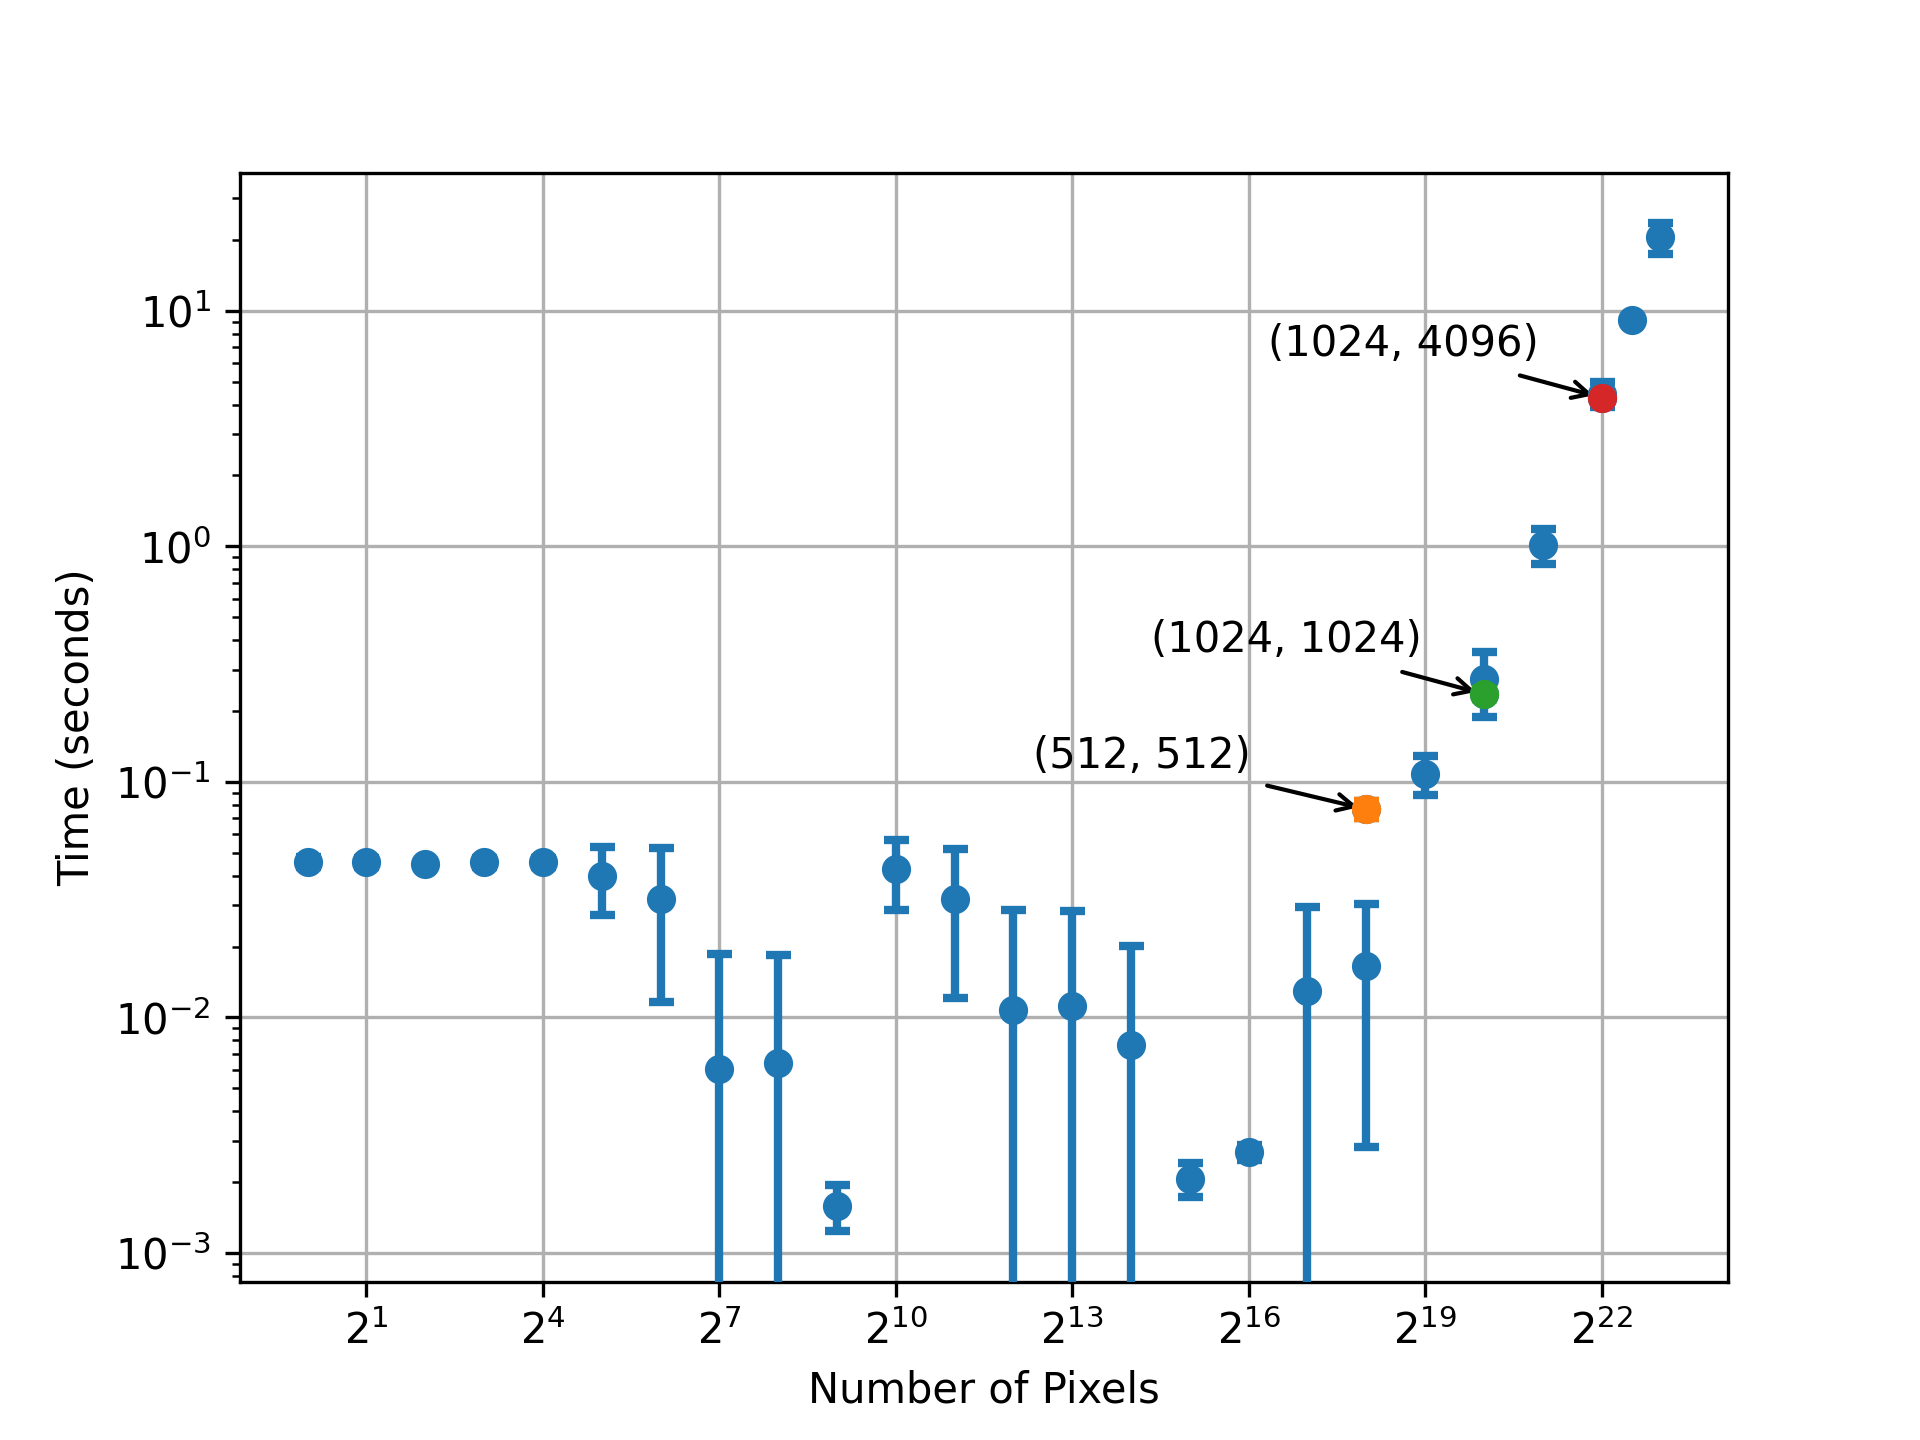
\includegraphics[width=.75\columnwidth]{figures/scaling/scaling}
	\caption{\label{si:fig:scaling} Scaling of transport time as a function of number of pixels for 32-bit integer arrays. Both the x- and y-axes are logarithmically scaled. Common camera sizes (512, 512), (1024, 1024), and (1024, 4096) are highlighted to provide context for camera users.}
\end{figure}

Common camera sizes (512, 512), (1024, 1024), and (1024, 4096) are highlighted in \ref{si:fig:scaling} to provide context.

There are some strategies that could be used to mitigate the performance problems of large cameras, but they have not been implemented because large arrays remain an edge case among current \yaq{} users.
Such strategies could include enabling compression, using transport layers other than TCP, using regions-of-interest (ROIs) to limit array sizes, and writing arrays locally to disk and providing mechanisms for retrieval out of band.
The Avro Specification \cite{AvroSpecification} specifically provides for compression codecs in the case of storing to disk, but there is nothing preventing the RPC pipe from similarly encoding the data, provided both ends of the communication support it.
This would allow larger arrays to be transported using fewer bytes over TCP, which would likely improve performance for large arrays where TCP transport is the bottleneck.
While TCP is the only currently supported transport layer for \yaq{}, this limitation could be lifted in the future.
TCP was chosen as the preferred starting point because it is ubiquitous, being available on every desired platform and implementation language.
One alternative that would be relatively easy to support would be Unix domain sockets (UDS).
UDS has an extremely similar interface to TCP sockets, and are handled in Python by the same standard library module.
UDS is potentially more performant, but as the name suggests are limited to Unix-like systems (i.e. it will not work on Windows).
ROIs are implemented on the handful of cameras currently in the \yaq{} ecosystem \cite{yaqd_andor,yaqd_pi}, however we are still in the experimentation phase and have not standardized ROI configuration into a \yaq{} trait.
When only a subset of the total camera area is interesting, this is one way to limit array size over the interface.
Finally \yaq{} daemons could be implemented to write arrays locally to disk, rather than transferring over the \yaq{} interface directly.
This has not yet been implemented, and would require clients to have knowledge of how to retrieve and display the images collected, but there is nothing preventing this if throughput is a limitation.
If such behavior became a standard feature desired for cameras, it should be encapsulated in a \yaq{} trait to provide a consistent interface.

To reproduce this figure, you will need the libraries specified in ``figures/requirements.txt''.
The scripts for generating this figure, including the \yaq{} daemon, are located in ``figures/scaling''.
To generate the data, run the \yaq{} daemon using \texttt{python scaling.py --config config.toml} from with in the ``scaling'' folder.
Then run \texttt{python scaling-data-gen.py}, which will communicate with the running daemon and produce a CSV written to standard out.
The result can be saved to \texttt{scaling.csv}.
To visualize the results, run \texttt{python plot-scaling.py}, which will read the CSV and produce the image.

\section{Package size analysis}

The raw data for package size analysis was collected using Tokei\cite{tokei}, a command line tool for analysing line lengths of source code.
It includes breaking down line length into ``code'', ``comments'', and ``blank'' lines.
The package size data was curated into \texttt{figures/lines\_histogram.txt}, which includes annotations as to the ``type'' and ``class'' for each file.
The ``type'' annotation is one of ``stub'' (meaning that the bulk of the implementation is in another file), ``normal'' (an individual daemon with the bulk of its implementation), ``protocol'' (an implementation the provides for multiple daemons, such as those referred to by ``stub''s, or ``serial'' (the implementation of a serial protocol rather than a full fledged daemon).
The ``class'' refers to the primary function of the daemon and is one of the following values: ``is-sensor'' for detectors, ``has-position'' for setable hardware, ``serial'' (identical to ``type'' annotation), and ``other'' for daemons which do not fit in the above categories.

The plotting script \texttt{figures/lines\_histogram.py} can be used to generate the figure from this text file.
The figure uses the ``code'' lines to generate a histogram of file sizes in the \yaq{} python implementations.
This is a measurable proxy for the amount of work that implementing an individual \yaq{} daemon entails, though of course cannot capture the work involved in learning the lower level interface.

\clearpage

\printbibliography

\end{document}
